\clearpage
\subsection{Long-slit spectroscopy, N band}
\label{ssec:recipes_lss_n}
A draft of the reduction cascade is shown in
Fig.~\ref{Fig:NLssAssomap} together with the data processing table
(Table~\ref{Tab:NLssDatProc}). The first part aims to update the static calibration database, in particular the creation of the gain map (\REC{met_det_lingain}) and the determination of the \ac{ADC} slitlosses (\REC{met_LM_adc_slitloss}). Both are executed only when an update is required, e.g. after a major instrument interention or on yearly basis. The second part comprises the basic
calibrations, e.g. the 
dark correction and the spectroscopic flatfielding via \ac{RSRF}, followed by the third part, the main calibration steps, incorporating the wavelength calibration (by means of atmospheric lines visible in the respective spectra and the first guess wavelength solution created during \ac{AIT}) and the determination of the response curve for the flux calibration. Therefore the main step of the wavelength calibration is carried out in the recipes \REC{met_LM_lss_flux} and \REC{met_LM_lss_sci}. Finally, the telluric absorption correction is applied using the modelling approach with \texttt{molecfit}.
%------------------------------------------------------------------------------------------------------------------
\subsubsection{Recipes \REC{metis_det_lingain} and \REC{metis_det_dark}}
These recipes are described in Section~\ref{Sec:detector_calibration}.
%------------------------------------------------------------------------------------------------------------------
\subsubsection{Recipe \REC{metis_N_adc_slitloss}}
This recipe aims to determine the slit losses induced by the fixed \ac{ADC} positions. The recipe aims to create a table with slitlosses (\STATCALIB{N_ADC_SLITLOSS}), which is added to the static database and used in the recipes \REC{met_N_lss_flux} and \REC{met_N_lss_sci}. This recipe is to be carried out only when an update of the database is needed.

As the algorithm to determine the slitlosses is still TBD, we do not give more details here. More information can be found in the Section "Calibration of slit losses" in the Calibration Plan \cite{METIS-calibration_plan}. 

%------------------------------------------------------------------------------------------------------------------
\subsubsection{N-LSS Flatfielding recipe \REC{metis_N_lss_rsrf}:}\label{rec:lssnrsrf}
The recipe \REC{metis_N_lss_rsrf} aims to create a spectroscopic master flatfield for determining the pixel-to-pixel sensitivity and to enable the order location algorithm (\REC{metis_N_ss_trace}).
\begin{figure}[ht]
  \centering
  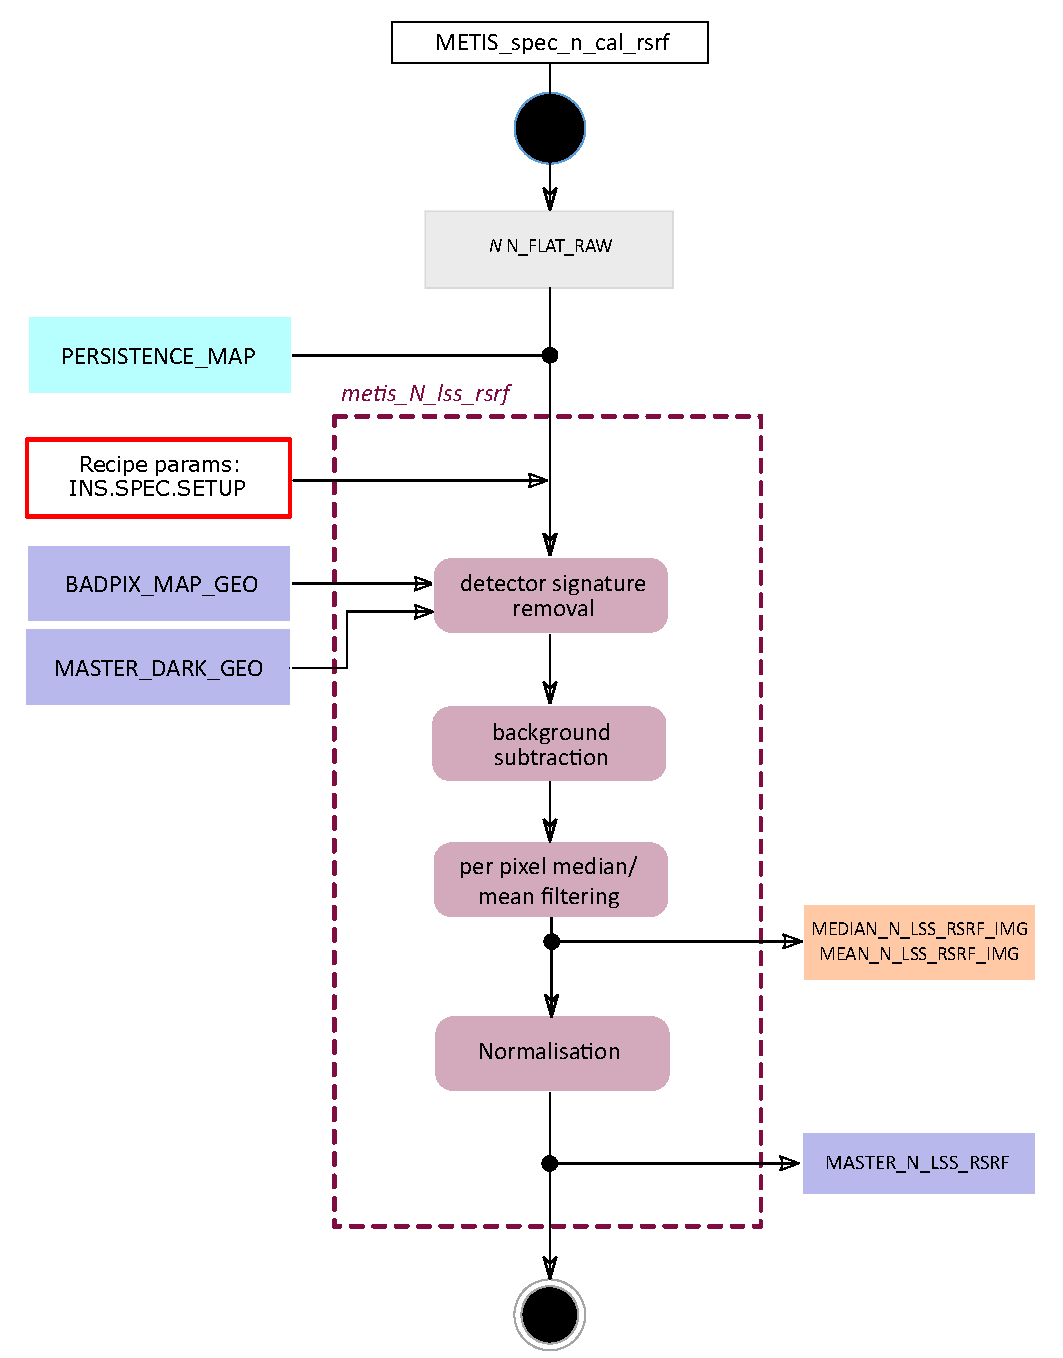
\includegraphics[width=0.5\textheight]{figures/metis_n_lss_rsrf_v0.72.pdf}
  \caption[Recipe: \REC{metis_N_lss_rsrf}]{\REC{metis_N_lss_rsrf} --
    Spectroscopic faltfielding with \ac{RSRF}.}
  \label{Fig:rec_n_lss_rsrf}
\end{figure}

\begin{recipedef}
Name:		& \REC{metis_N_lss_rsrf} \\
Purpose:	& Spectroscopic flatfielding with \ac{RSRF} \\
Type:		& Calibration\\
Requirements: & TBD \\
Observing templates: & None \\
Input data:     & $N\times$ \FITS{N_RSRF_RAW} \\
Parameters: 	& TBD\\
Algorithm:      & median/mean filtering\\
                & normalisation\\
Output data:	& \PROD{MASTER_N_LSS_RSRF} (\FITS{PRO.CATG=MASTER_N_LSS_TRSRF}): \\
Expected accuracies: & (TBD)\\
QC1 parameters: & \QC{TBD}: TBD\\
\end{recipedef}

\clearpage
\subsubsection{N-LSS Order detection \REC{metis_N_lss_trace}:}\label{rec:lssNtrace}
The recipe \REC{metis_N_lss_trace} aims at detecting the orders and a polynomial fitting of the order locations (see \cite{pis02} and \cite{pis21} for details on the algorithms).

\begin{figure}[ht]
  \centering
  \includegraphics[width=0.5\textheight]{figures/metis_N_lss_trace_v0.74.pdf}
  \caption[Recipe: \REC{metis_N_lss_trace}]{\REC{metis_N_lss_trace} --
    Detection and polynomial fitting of the order location.}
  \label{Fig:rec_N_lss_wave}
\end{figure}

\begin{recipedef}
Name:		& \REC{metis_N_lss_trace} \\
Purpose:	& Detection of order location \\
Type:		& Calibration\\
Requirements: & TBD \\
Observing templates: & None \\
Input data:     & \PROD{MASTER_N_LSS_RSRF} \\
Parameters: 	& polynomial degree\\
Algorithm:      & Detection of the order edges\\
                & Polynomial fitting\\
Output data:	& \PROD{N_LSS_TRACE} (\FITS{PRO.CATG=N_LSS_TRACE}): Polynomial coefficients\\
Expected accuracies: & (TBD)\\
QC1 parameters: & \QC{TBD}: TBD\\
\end{recipedef}

\clearpage

%------------------------------------------------------------------------------------------------------------------
\subsubsection{N-LSS flux calibration recipe \REC{metis_N_lss_flux}:}\label{rec:lssNflux}
Flux calibration with spectrophotometric standard stars: As first step the detector master calibration files derived previously are applied followed by the background subtraction, if needed the distortion correction (\PROD{N_DIST_SOL}), and
the wavelength calibration by means of the first guess solution (\PROD{N_WAVE_GUESS}) and the telluric sky lines (c.f. Sect.\,8.5 in \cite{DRLS}). Then the recipe extracts the standard star spectrum object, removes sky lines, collapses the 2D to 1D spectra and applies a telluric correction in an automated way to the standard star spectrum (in contrast to the science observations, which are telluric corrected in a dedicated recipe to achieve the best correction). The response curve is obtained by comparing the extracted spectrum with a model and/or another reference spectrum of the standard star. Currently it is foreseen to use the same standard stars as in \ac{CRIRES}/CRIRES+ and \ac{VISIR}. It is under investigation whether more stars are needed.
\begin{figure}[ht]
  \centering
  \includegraphics[width=0.4\textheight]{figures/metis_N_lss_flux_v0.72.pdf}
  \caption[Recipe: \REC{metis_N_lss_flux}]{\REC{metis_N_lss_flux} --
    Flux calibration recipe.}
  \label{Fig:rec_N_lss_flux}
\end{figure}
\clearpage
\begin{recipedef}
Name:		& \REC{metis_N_lss_flux} \\
Purpose:	& Flux calibration \\
Type:		& Calibration\\
Requirements: & METIS-6084, METIS-6074 \\
Observing templates: & \TPL{METIS_spec_N_acq}, \\
                & \TPL{METIS_spec_N_cal_lampwave}\\
                & \TPL{METIS_spec_N_cal_AutoNodOnSlit}, \\
                & \TPL{METIS_spec_N_obs_GenericOffset} \\
                & \TPL{METIS_spec_N_cal_standard}\\
                & \TPL{METIS_spec_N_cal_slit_adc}\\
Input data: 	& raw spectrophotometric STANDARD star data (\FITS{N_FLUX_RAW})\\
                & \EXTCALIB{PERSISTENCE_MAP} \\
                & \PROD{GAIN_MAP_GEO} \\
                & \PROD{BADPIX_MAP_GEO} \\
                & \PROD{MASTER_DARK_GEO} \\
                & \PROD{MASTER_N_LSS_RSRF} \\
                & \PROD{N_LSS_DIST_SOL} \\
                & \PROD{N_WAVE_GUESS} \\
                & \EXTCALIB{AO_PSF_MODEL} \\
                & \STATCALIB{ATM_LINE_CAT} \\
                & \STATCALIB{HITRAN}, \STATCALIB{LSF_KERNEL}, \EXTCALIB{ATM_PROFILE}\\
                & \STATCALIB{REF_FLUX_CAT} \\
Parameters: 	& (TBD)\\
Algorithm:      & Application of master calibration files\\
                & Background removal\\
                & Determination and application of the distortion correction\\
                & Determination and application of the wavelength solution\\
                & Identifying/separatiing sky/object pixels\\
                & Removing sky lines: Creation and Subtraction of 2D sky\\
                & Collapsing 2D to 1D spectrum, (see Fig.\,\ref{Fig:rec_N_lss_sci})\\
                & Determination and application of response curve\\
Output data:	& \PROD{N_STD_OBJ_MAP}: Pixel map of object pixels\\
            	& \PROD{N_STD_SKY_MAP}: Pixel map of sky pixels\\
                % & \PROD{N_STD_2D}: coadded, wavelength calibrated 2D spectrum\\
              	& \PROD{N_STD_1D}: coadded, wavelength calibrated, collapsed 1D spectrum\\
                & \PROD{INSTR_RESPONSE}: response function (TBD)\\
            %     & \PROD{N_SCI_SLIT} (\FITS{PRO_CATG=N_LSS_2D_WAVE}): background corrected 2d spectra \\
            %     & \PROD{N_SCI_OBJ_MAP}: Pixel map of object pixels\\
            % 	& \PROD{N_SCI_SKY_MAP}: Pixel map of sky pixels\\
            %     % & \PROD{N_SCI_2D}: coadded, wavelength calibrated 2D spectrum\\
            %     % & (\FITS{PRO_CATG}: \FITS{N_LSS_2d_coadd_wavecal}) \\
            %     % & (\FITS{PRO_CATG}: \FITS{N_LSS_1d_coadd_wavecal}) \\
            %   	& \PROD{N_SCI_FLUX_2D}: coadded, wavelength and flux calibrated 2D spectrum\\
            %     & (\FITS{PRO_CATG}: \FITS{N_LSS_2d_coadd_wavecal_flux}) \\
            %   	& \PROD{N_SCI_FLUX_1D}: coadded, wavelength and flux calibrated 1D spectrum\\
            %     & (\FITS{PRO_CATG}: \FITS{N_LSS_1d_coadd_wavecal_flux}) \\
            %     & \PROD{N_WAVE_GUESS} (\FITS{PRO.CATG=N_WAVE_GUESS}): Wavelength solution\\
            %     & \PROD{N_DIST_SOL} (\FITS{PRO.CATG=N_DIST_SOL}): Distortion solution\\
Expected accuracies: & (TBD)\\
QC1 parameters: & \QC{QC N LSS STD BACKGD MEAN}: Mean value of background\\
                & \QC{QC N LSS STD BACKGD MEDIAN}: Median value of background\\
                & \QC{QC N LSS STD BACKGD SIGMA}: Sigma value of background\\
                & \QC{QC N LSS STD SNR}: Signal-to-noise ration of flux standard star spectrum\\
                & \QC{QC N LSS STD SNRNOISE}: Noise level of flux standard star spectrum\\
                & \QC{QC N LSS STD FWHM}: FWHM of flux standard spectrum\\
                & \QC{N LSS FLUX}: (TBdef) \\
                & \QC{QC N LSS FLUX WAVECAL DEVMEAN}: Mean deviation from the
                  wavelength reference frame (TBDef)\\
                & \QC{QC N LSS FLUX WAVECAL FWHM}: Measured FWHM of lines\\
                & \QC{QC N LSS FLUX WAVECAL NIDENT}: Number of identified lines\\
                & \QC{QC N LSS FLUX WAVECAL NMATCH}: Number of lines matched between
                    catalaogue and spectrum\\
                & \QC{QC N LSS FLUX WAVECAL POLYDEG}: Degree of the polynomial\\
                & \QC{QC N LSS FLUX WAVECAL POLYCOEFF\<n\>}: $n$-th coefficient of the polynomial\\
                & \QC{QC N LSS FLUXCAL SNR}: Signal-to-noise ration of flux standard star spectrum\\
                & \QC{QC N LSS FLUXCAL SNRNOISE}: Noise level of flux standard star spectrum\\
                & \QC{QC N LSS FLUXCAL FWHM}: FWHM of flux standard spectrum\\
                & \QC{QC N LSS FLUXCAL PSFLOSS}: percentage of AO induced slit losses (TBdef)\\
\end{recipedef}

\subsubsection{N-LSS science reduction recipe \REC{metis_N_lss_sci}:}
The science calibration recipe comprises the extraction of the object (i.e. separation of object/sky pixels), removing the sky lines, the application of the response curve previously defined, the 2D to 1D collapse and the coaddition. In contrast to the flux standard star reduction, the telluric correction on the science data is done in a dedicated recipe afterwards to achieve best quality for the correction.
\begin{figure}[ht]
  \centering
  \includegraphics[width=0.4\textheight]{figures/metis_N_lss_sci_v0.72.pdf}
  \caption[Recipe: \REC{metis_N_lss_sci}]{\REC{metis_N_lss_sci} --
    Science reduction recipe.}
  \label{Fig:rec_N_lss_sci}
\end{figure}
\clearpage

\begin{recipedef}
Name:		& \REC{metis_N_lss_sci} \\
Purpose:    Science data calibration\\
Type:		& Science reduction\\
Requirements: & METIS-6084 \\
Observing templates: & \TPL{METIS_spec_N_acq}, \\
                & \TPL{METIS_spec_N_obs_AutoNodOnSlit}, \\
                & \TPL{METIS_spec_N_obs_GenericOffset} \\
                & \TPL{METIS_spec_N_cal_slit_adc}\\
Input data: 	&  \PROD{N_LSS_SCI_WAVE}\\
Input data: 	& raw SCIENCE data (\FITS{N_SCI_RAW})\\
                & \EXTCALIB{PERSISTENCE_MAP} \\
                & \PROD{GAIN_MAP_GEO} \\
                & \PROD{BADPIX_MAP_GEO} \\
                & \PROD{MASTER_DARK_GEO} \\
                & \PROD{MASTER_N_LSS_RSRF} \\
                & \PROD{N_LSS_DIST_SOL} \\
                & \PROD{N_WAVE_GUESS} \\
                & \STATCALIB{ATM_LINE_CAT} \\
                & \EXTCALIB{AO_PSF_MODEL} \\
                & \PROD{INSTR_RESPONSE} \\
Parameters: 	& (TBD)\\
Algorithm:      & Application of the detector master calib files\\
                & wavelength calibration \\
                & Identifying/separatiing sky/object pixels\\
                & Removing sky lines: Creation and Subtraction of 2D sky\\
                & Coaddition of individual object spectra of one OB\\
                & Collapsing 2D to 1D spectrum, (see Fig.\,\ref{Fig:rec_N_lss_sci})\\
                & Application of the response function (flux calibration) \\
Output data:	& \PROD{N_SCI_OBJ_MAP}: Pixel map of object pixels\\
            	& \PROD{N_SCI_SKY_MAP}: Pixel map of sky pixels\\
                & \PROD{N_LSS_SCI_2D}: coadded, wavelength calibrated 2D spectrum\\
                & (\FITS{PRO_CATG}: \FITS{N_LSS_2d_coadd_wavecal}) \\
              	& \PROD{N_LSS_SCI_1D}: coadded, wavelength 1D spectrum\\
                & (\FITS{PRO_CATG}: \FITS{N_LSS_1d_coadd_wavecal}) \\
                & \PROD{N_LSS_SCI_FLUX_2D}: coadded, wavelength calibrated 2D spectrum\\
                & (\FITS{PRO_CATG}: \FITS{N_LSS_2d_coadd_wavecal}) \\
              	& \PROD{N_LSS_SCI_FLUX_1D}: coadded, wavelength 1D spectrum\\
                & (\FITS{PRO_CATG}: \FITS{N_LSS_1d_coadd_wavecal}) \\
Expected accuracies: & (TBD)\\
QC1 parameters: & \QC{QC N LSS SCI SNR}: Signal-to-noise ration of science spectrum\\
                & \QC{QC N LSS SCI SNRNOISE}: Noise level of science spectrum\\
                & \QC{QC N LSS SCI FLUX SNR}: Signal-to-noise ration of flux calibrated  science spectrum\\
                & \QC{QC N LSS SCI FLUX SNRNOISE}: Noise level of flux calibrated science spectrum\\
                & \QC{N LSS SCI}: (TBdef) \\
                & \QC{QC N LSS SCI WAVECAL DEVMEAN}: Mean deviation from the
                  wavelength reference frame (TBDef)\\
                & \QC{QC N LSS SCI WAVECAL FWHM}: Measured FWHM of lines\\
                & \QC{QC N LSS SCI WAVECAL NIDENT}: Number of identified lines\\
                & \QC{QC N LSS SCI WAVECAL NMATCH}: Number of lines matched between
                    catalaogue and spectrum\\
                & \QC{QC N LSS SCI WAVECAL POLYDEG}: Degree of the polynomial\\
                & \QC{QC N LSS SCI WAVECAL POLYCOEFF\<n\>}: $n$-th coefficient of the polynomial\\
\end{recipedef}

\subsubsection{N-LSS telluric correction recipe \REC{metis_N_lss_mf_model}:}\label{rec:N_LSS_mf_model}
blah

\begin{figure}[ht]
  \centering
  \includegraphics[width=0.5\textheight]{figures/metis_N_lss_mf_model_v0.72.pdf}
  \caption[Recipe: \REC{metis_N_lss_mf_model}]{\REC{metis_N_lss_mf_model} --
    TBD.}
  \label{Fig:rec_N_lss_mf_model}
\end{figure}
\clearpage

\begin{recipedef}
Name:		& \REC{metis_N_lss_mf_model} \\
Purpose:	& Achieve the best fit for modelling the transmission curve to be applied as telluric correction \\
Type:		& Post-calibration\\
Requirements: & METIS-4051, METIS-6091 \\
Observing templates: & None\\
Input data: 	& \PROD{N_LSS_SCI_FLUX_1D}\\
                & \EXTCALIB{LSF_Kernel} \\
                & \EXTCALIB{ATM_PROFILE} \\
                & \EXTCALIB{HITRAN} \\
Parameters: 	& \texttt{molecfit} parameters (c.f. \cite{molecfit})\\
Algorithm:      & Fit of telluric features visible in the science input spectrum\\
                & Determination of best-fit parameter set\\
Output data:	& \PROD{MF\_BEST\_FIT\_TAB}\\
Expected accuracies: & (TBD)\\
QC1 parameters: & \QC{TBD}: TBD\\
\end{recipedef}

\subsubsection{N-LSS telluric correction recipe \REC{metis_N_lss_mf_calctrans}:}\label{rec:N_LSS_mf_calctrans}
blah

\begin{figure}[ht]
  \centering
  \includegraphics[width=0.5\textheight]{figures/metis_N_lss_mf_calctrans_v0.72.pdf}
  \caption[Recipe: \REC{metis_N_lss_mf_calctrans}]{\REC{metis_N_lss_mf_calctrans} --
    TBD.}
  \label{Fig:rec_N_lss_mf_calctrans}
\end{figure}
\clearpage

\begin{recipedef}
Name:		& \REC{metis_N_lss_mf_calctrans} \\
Purpose:	& Calculation of the synthetic transmission \\
Type:		& Post-calibration\\
Requirements: & METIS-4051, METIS-6091 \\
Observing templates: & None\\
Input data: 	& \PROD{MF\_BEST\_FIT\_TAB}\\
                & \EXTCALIB{LSF_Kernel} \\
                & \EXTCALIB{ATM_PROFILE} \\
                & \EXTCALIB{HITRAN} \\
Parameters: 	& \texttt{molecfit} parameters (c.f.  \cite{molecfit})\\
Algorithm:      & Calculate the entire transmission curve by means of the best-fit parameters\\
Output data:	& \PROD{SYNTH_TRANSMISSION}\\
Expected accuracies: & (TBD)\\
QC1 parameters: & \QC{TBD}: TBD\\
\end{recipedef}

\subsubsection{N-LSS telluric correction recipe \REC{metis_N_lss_mf_correct}:}\label{rec:N_LSS_mf_correct}
blah

\begin{figure}[ht]
  \centering
  \includegraphics[width=0.5\textheight]{figures/metis_N_lss_mf_correct_v0.72.pdf}
  \caption[Recipe: \REC{metis_N_lss_mf_correct}]{\REC{metis_N_lss_mf_correct} --
    TBD.}
  \label{Fig:rec_N_lss_mf_correct}
\end{figure}
\clearpage

\begin{recipedef}
Name:		& \REC{metis_N_lss_mf_correct} \\
Purpose:	& Apply the synthetic transmission to the science spectra \\
Type:		& Post-calibration\\
Requirements: & METIS-4051, METIS-6091 \\
Observing templates: & None\\
Input data: 	& \PROD{N_LSS_SCI_FLUX_1D}\\
                & \PROD{SYNTH_TRANSMISSION}\\
Parameters: 	& None\\
Algorithm:      & Apply telluric correction, i.e. divide the input science spectrum\\
                & by the synthetic transmission\\
Output data:	& \\
Expected accuracies: & (TBD)\\
QC1 parameters: & \QC{TBD}: TBD\\
\end{recipedef}







